
%(BEGIN_QUESTION)
% Copyright 2007, Tony R. Kuphaldt, released under the Creative Commons Attribution License (v 1.0)
% This means you may do almost anything with this work of mine, so long as you give me proper credit

This Honeywell model UDC2500 controller needs to connect to a loop-powered pressure transmitter in such a way that it displays the amount of pressure in the process vessel, and outputs a signal to the 120 VAC alarm lamp if the process pressure becomes too great.  Alarm relay \#1 in the controller has been configured for a high-pressure trip point of 140 PSI:

$$\includegraphics[width=15.5cm]{i02541x01.eps}$$

Sketch all necessary connecting wires and tubes to make this a working system.  Note: you will need to add electrical power sources to the diagram!  Also, identify the proper open/closed state for each hand valve contained in the pressure transmitter's three-valve isolation manifold.

\vskip 20pt \vbox{\hrule \hbox{\strut \vrule{} {\bf Suggestions for Socratic discussion} \vrule} \hrule}

\begin{itemize}
\item{} A problem-solving technique useful for making proper connections in pictorial circuit diagrams is to first identify the directions of all DC currents entering and exiting component terminals, as well as the respective voltage polarity marks (+,$-$) for those terminals, based on your knowledge of each component acting either as an electrical {\it source} or an electrical {\it load}.  Discuss and compare how these arrows and polarity marks simplify the task of properly connecting wires between components. 
\item{} Supposing the transmitter outputs a current value of 14 mA, calculate all voltage drops in this circuit.
\end{itemize}

\underbar{file i02541}
%(END_QUESTION)





%(BEGIN_ANSWER)

\noindent
{\bf Partial answer:}

$$\includegraphics[width=15.5cm]{i02541x02.eps}$$

%(END_ANSWER)





%(BEGIN_NOTES)

The second analog input (and its 250 ohm resistor) are extraneous to the solution.

$$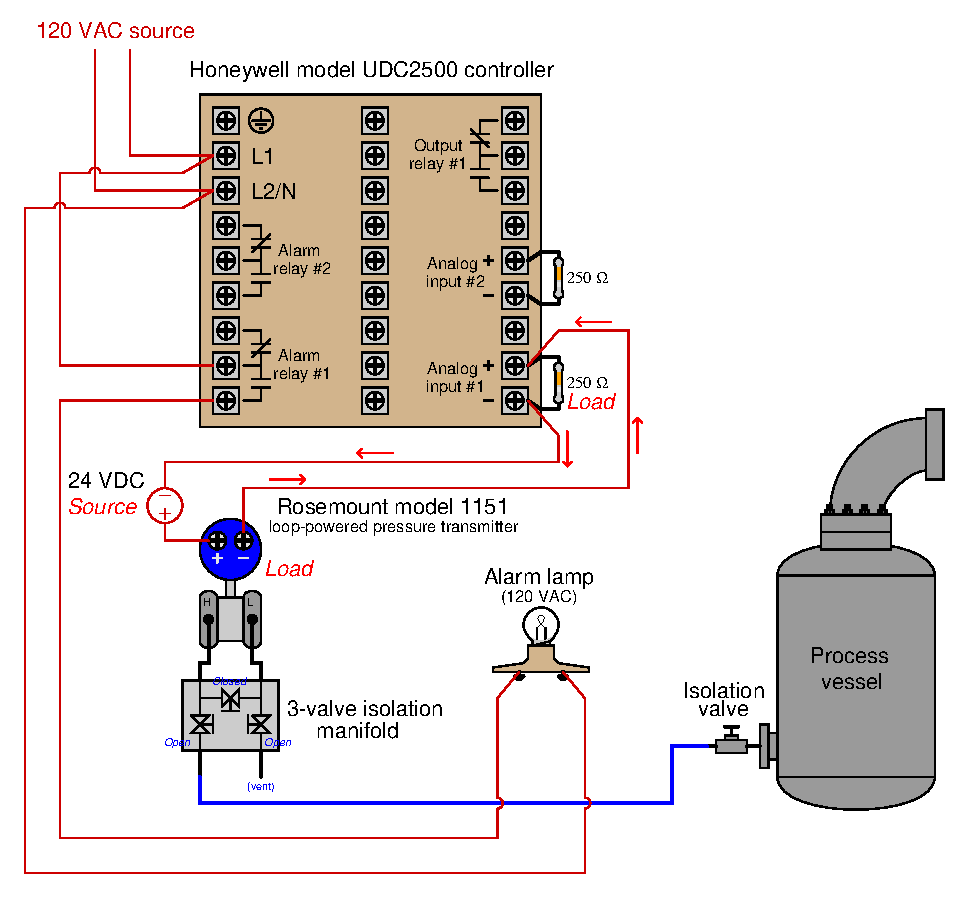
\includegraphics[width=15.5cm]{i02541x03.eps}$$

%INDEX% Pictorial circuit review (4-20 mA loop)

%(END_NOTES)


